\section{Co-diseño hardware/software: estudio histórico}
\label{sec:codisenio}
La auditoría recuperó del commit \texttt{66eede4} el estudio comparativo de
SMA10 anterior a la política final. Se comparan la misma estrategia y la misma
serie de 20\,000 ticks a 25 MHz: software, instrucción \texttt{custom-0} y
periférico MMIO. Son mediciones históricas, no nuevas ejecuciones de la versión
Momentum32. Los CSV resumidos, informe original y manifiesto de procedencia
están en \path{docs/evidencia_codisenio/}; los programas, RTL, testbenches y
trazas completas se conservan en ese commit del repositorio.

\subsection{Kernel, alternativas y recursos}
El perfil original identifica 163,93 ciclos medios en SMA10. El kernel ampliado
de historial, SMA y señal ocupa 186,62 de 218,66 ciclos/tick. La instrucción
\texttt{smaupd} fusiona la actualización $rd\leftarrow rd-rs1+rs2$ y añade un
tercer puerto de lectura de registros. El periférico MMIO conserva diez precios
y actualiza la suma al recibir cada byte; Espino sigue decidiendo la operación.

\begin{center}\small\begin{tabular}{lrrrrrr}\toprule
Variante & LUT4 & LC/1280 & BRAM/16 & Fmax (MHz) & Ciclos medios & CPI \\\midrule
Software & 980 & 1200 & 12 & 42,60 & 218,66 & 2,379 \\
custom-0 & 1133 & 1350 & 14 & No enruta & 70,73 & 2,286 \\
MMIO SMA10 & 1055 & 1279 & 13 & 40,50 & 60,64 & 2,259 \\\bottomrule
\end{tabular}\end{center}
Las LC combinan funciones de LUT y registro; se presentan separadas de LUT4.
\texttt{custom-0} excede el dispositivo por 70 LC: no tiene Fmax válida de
enrutado ni se considera una opción programable en HX1K. MMIO sí cabe, pero
el diseño de aquella etapa dejaba solo una LC libre.

\subsection{Ops/s y ley de Amdahl}
Aquí una operación útil es procesar un tick y escribir DECISION. La capacidad
del core es $25\cdot10^6/C$ ticks/s, con $C$ ciclos medios por tick. El estímulo
histórico llegaba cada 30 microsegundos, limitando el caudal a 33\,333 ticks/s.
Capacidad de servicio y caudal de entrada son magnitudes distintas.

\begin{center}\small\begin{tabular}{lrrrrr}\toprule
Variante & IC medios & Ciclos máx. & Capacidad (ticks/s) & Speedup & Amdahl \\\midrule
Software & 91,92 & 412 & 114\,331 & 1,000 & 1,000 \\
custom-0 & 30,94 & 266 & 353\,435 & 3,091 & 3,076 \\
MMIO SMA10 & 26,85 & 255 & 412\,270 & 3,606 & 3,692 \\\bottomrule
\end{tabular}\end{center}
Se usa $P=186,62425/218,6635\simeq0,8535$ y
\[
S_{\mathrm{Amdahl}}=\frac{1}{(1-P)+P/S_k},\qquad
S_k=\frac{186,62425}{C_{k,\mathrm{variante}}}.
\]
Los kernels medidos de custom-0 y MMIO son 39,04 y 27,18 ciclos, respectivamente.
Su perfil regional usa 100 ticks; los tiempos totales y el speedup observado
usan 20\,000. Esa diferencia de muestra y el trabajo fuera del kernel explican
que la predicción no coincida exactamente con el speedup total.

\subsection{Roofline simplificado y decisión final}
Para el roofline, operación significa suma/resta entera, no tick. El modelo
supone pico de 25 Mops/s, ancho de banda de BRAM de 50 MB/s y
$P(I)=\min(25,50I)$ Mops/s. Se excluyen tráfico de instrucciones, polling y
control; el ancho de banda es un supuesto de arquitectura, no una medición.

\begin{center}\small\begin{tabular}{lrrrr}\toprule
Kernel & Operaciones & Bytes/tick & Intensidad (ops/B) & Techo (Mops/s) \\\midrule
Software & 14 & 41 & 0,341 & 17,07 \\
custom-0 & 6 & 5 & 1,200 & 25,00 \\
MMIO SMA10 & 6 & 11 & 0,545 & 25,00 \\\bottomrule
\end{tabular}\end{center}
\begin{center}
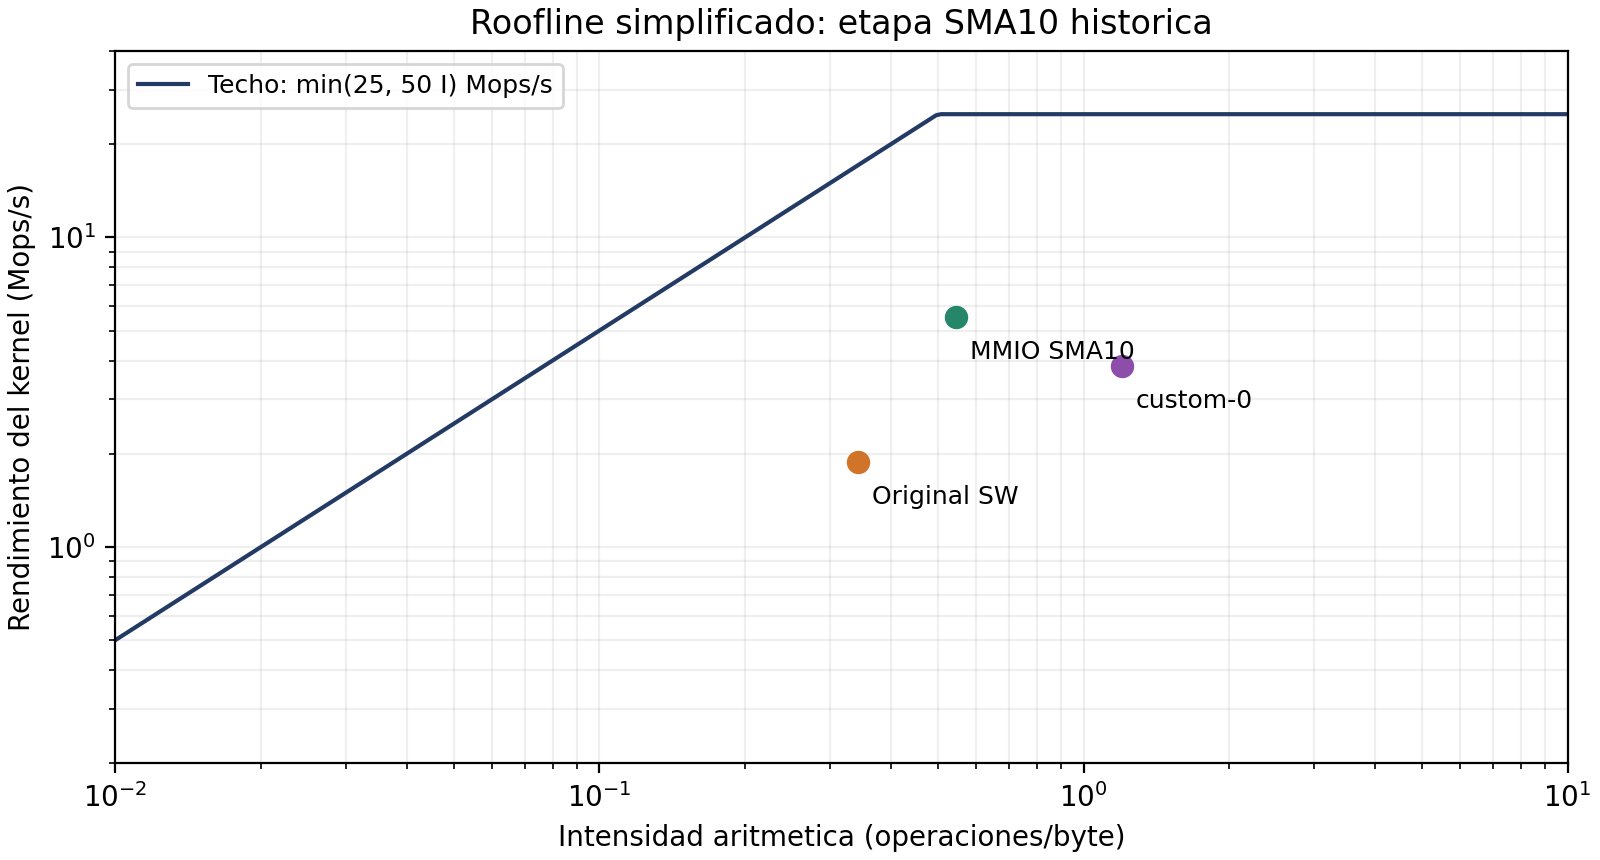
\includegraphics[width=0.88\linewidth]{figuras/roofline_historico.png}
\end{center}
Los puntos combinan los conteos aproximados declarados y la latencia regional
medida; no son pruebas de ancho de banda ni una caracterización del firmware
final. El kernel software queda bajo el techo de memoria del modelo, mientras
las dos alternativas se ubican bajo el techo de cómputo.

El estudio justifica descartar custom-0 por área y conservar MMIO como opción
implementable. La integración final cambia la política a Momentum32 con stop
y reduce el reloj del SoC a 12,5 MHz para usar el arranque validado. SUM10 sigue
presente, pero no participa en la regla final: no corresponde atribuirle un
speedup de 3,606 a Momentum32. Su evaluación propia está en la sección de
latencia y ocupa \Celdas\ LC y \Bram\ BRAM. Falta un perfil regional y una
comparación de variantes bajo la misma política final para cerrar esa extensión
del estudio sin mezclar mejoras de algoritmo y mejoras de hardware.
